% Drawing 154/01-12 -- folder 154, batch 01, archive page 18 (PDF page 19).
% Transcription: figures : un faisceau orange coupant une droite jaune, recouvert d'une spirale au crayon qui s'allonge vers la droite (le secteur est hachuré) ; au-dessous, une droite orange $\Delta_{i_0}$ traversée de quatre faisceaux, et une droite jaune $D$ qui la longe d'un côté puis, franchissant le sommet marqué d'un gros point, passe de l'autre côté, la bande entre elles étant hachurée
% Kind: pencil under a pencil spiral; line crossed by four pencils with a line D changing sides. Method 2 (schematic redraw from the facsimile). Status: partial.
% Notes: Two figures in the left column. Top: a pencil of orange lines cutting a yellow line, covered by a pencil spiral of loops drawn out to the right; the spiral is approximate (loop count and shape) and the hatching of the sector under it is left out. Bottom: the orange line Delta_{i0} crossed by four pencils (and two single strokes); the yellow line D runs along one side of it, crosses at the vertex marked with a large point, and runs along the other side; the band between them is hatched. Read from the page view only (no zoom).
% Coordinates: 1 unit = 1 mm = 1/100 of the crop width (bbox in page fractions: [0.13, 0.271, 0.61, 0.457]).
% Redrawn by Claude (claude-opus-5-5), issue #73, 2026-11-07; not checked by a human; not compiled (no TeX in the session).
% Rights: reproduces part of the work -- behind RENDER_TRANSCRIPTS, never published by itself.
\documentclass[tikz,border=3pt]{standalone}
\usepackage{amsmath,amssymb}
\usetikzlibrary{patterns,arrows.meta}
\tikzset{Or/.style={orange!90!black}, Ye/.style={yellow!80!orange}, Lg/.style={green!60!black!70}, Dg/.style={green!45!black}, Br/.style={brown!80!black}, Rd/.style={red!85!black}, Bl/.style={blue!70!black}, Gy/.style={black!40}, pencil/.style={black!45}, struck/.style={black!35}, mark/.style={circle,draw,inner sep=1.3pt}, pt/.style={circle,fill,inner sep=0.9pt}, opt/.style={circle,draw,fill=white,inner sep=1.1pt}}
\begin{document}
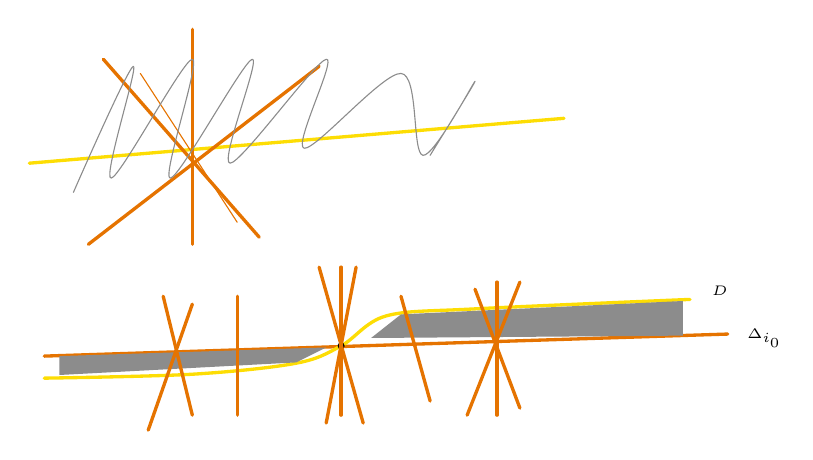
\begin{tikzpicture}[x=1mm,y=1mm,line cap=round,line join=round,font=\scriptsize]
\draw[Ye,very thick] (1.9,-18.9) -- (69.8,-13.2);
\draw[Or,very thick] (9.4,-29.2) -- (38.7,-6.6);
\draw[Or,very thick] (22.6,-1.9) -- (22.6,-29.2);
\draw[Or,very thick] (11.3,-5.7) -- (31.1,-28.3);
\draw[Or] (16,-7.5) -- (28.3,-26.4);
\draw[pencil] plot[smooth, tension=0.55] coordinates {(7.5,-22.6) (15.1,-6.6) (12.3,-20.8) (22.6,-5.7) (19.8,-20.8) (30.2,-5.7) (27.4,-18.9) (39.6,-5.7) (36.8,-17) (49.1,-7.5) (51.9,-17.9) (58.5,-8.5) (52.8,-17.9)};
\draw[Or,very thick] (3.8,-43.4) -- (90.6,-40.6);
\node[inner sep=1pt] at (95.3,-41.1) {\tiny $\Delta_{i_0}$};
\draw[Ye,very thick] plot[smooth, tension=0.55] coordinates {(3.8,-46.2) (22.6,-45.7) (35.8,-44.3) (41.5,-42.1) (47.2,-38.3) (58.5,-37.4) (85.8,-36.2)};
\node[inner sep=1pt] at (89.6,-35.1) {\tiny $D$};
\node[pt] at (41.5,-42.1) {};
\fill[pattern=north east lines,pencil] (5.7,-43.4) -- (39.6,-42.3) -- (35.8,-44.2) -- (5.7,-45.8) -- cycle;
\fill[pattern=north east lines,pencil] (45.3,-41.1) -- (84.9,-40.8) -- (84.9,-36.4) -- (49.1,-38.1) -- cycle;
\draw[Or,very thick] (17,-52.8) -- (22.6,-36.8);
\draw[Or,very thick] (18.9,-35.8) -- (22.6,-50.9);
\draw[Or,very thick] (28.3,-35.8) -- (28.3,-50.9);
\draw[Or,very thick] (38.7,-32.1) -- (44.3,-51.9);
\draw[Or,very thick] (43.4,-32.1) -- (39.6,-51.9);
\draw[Or,very thick] (41.5,-32.1) -- (41.5,-50.9);
\draw[Or,very thick] (49.1,-35.8) -- (52.8,-49.1);
\draw[Or,very thick] (57.5,-50.9) -- (64.2,-34);
\draw[Or,very thick] (61.3,-34) -- (61.3,-50.9);
\draw[Or,very thick] (58.5,-34.9) -- (64.2,-50);
\end{tikzpicture}
\end{document}
